\documentclass[a4paper,12 pt]{article}
\usepackage{color}
\usepackage[indonesian]{babel}
\usepackage{graphicx}
\graphicspath{ {./images/} }
\usepackage{blindtext}

\setlength{\parindent}{150pt}


\pagenumbering{arabic}

%membuat url bisa diklik
\usepackage{hyperref}
\hypersetup{
    colorlinks,
    citecolor=black,
    filecolor=black,
    linkcolor=blue,
    urlcolor=blue
}

\title{\textbf{Tugas Perorangan }\linebreak 
\textbf{Prosedur Perpustakaan}\linebreak}
\date{}


\begin{document}

\maketitle
\thispagestyle{empty}
\begin{center}

\includegraphics[width=8cm,height=6cm]{logo}
\end{center}


\vspace{0.5 cm}
\begin{center}
\begin{tabular}{ll}
Nama & : Rifqi Fadil Fahrial \\
NIM & : 1222646\\
\end{tabular}
\newline
\newline
\newline
Mata Kuliah: Rekayasa Perangkat Lunak \\
Dosen Pengampu: Mina Ismu Rahayu, M.T \linebreak
\newline
\newline
\textbf {TEKNIK INFORMATIKA} \\
\textbf {FAKULTAS INFORMATIKA} \\
\textbf {STMIK BANDUNG}
\linebreak
\textbf {2024} \linebreak
\end{center}

\pagebreak

\tableofcontents
\clearpage

\section{Prosedur Pendaftaran}
\begin{enumerate}
  \item Pendaftar menanyakan prosedur pendaftaran kepada penjaga perpustakaan
  \item Penjaga perpustakaan memberikan form pendaftaran kepada pendaftar
  \item pendaftar mengisi form pendaftaran dengan data-data yang diperlukan
  \item pendaftar memberikan form pendaftaran yang sudah diisi kepada penjaga perpustakaan
  \item penjaga perpustakaan memeriksa isi dari form pendaftaran apakah si pendaftar sudah memasukan data dengan sesuai atau tidak
  \item jika ditemukan data ghang tiedak benar maka form dikembalikan kepada si pendaftar untuk mengubah datanya agar benar dan sesuai
  \item jika semua data telah diisi dengan benar maka penjaga perpustakaan menginput ke dalam database perpustakaan untuk memasukan nama pendaftar sebagai anggota perpustakaan yang sah 
  \item jika data yang diinput terjadi konflik dengan data yang telah ada (duplikasi) maka penjaga perpustakaan menanyakan apakah pengguna telah mendaftar sebelumnya atau belum, jika iya maka petugas perpustakaan menyarankan pendaftar untuk menggunakan data yang sudah ada 

\end{enumerate}

\begin{center}
  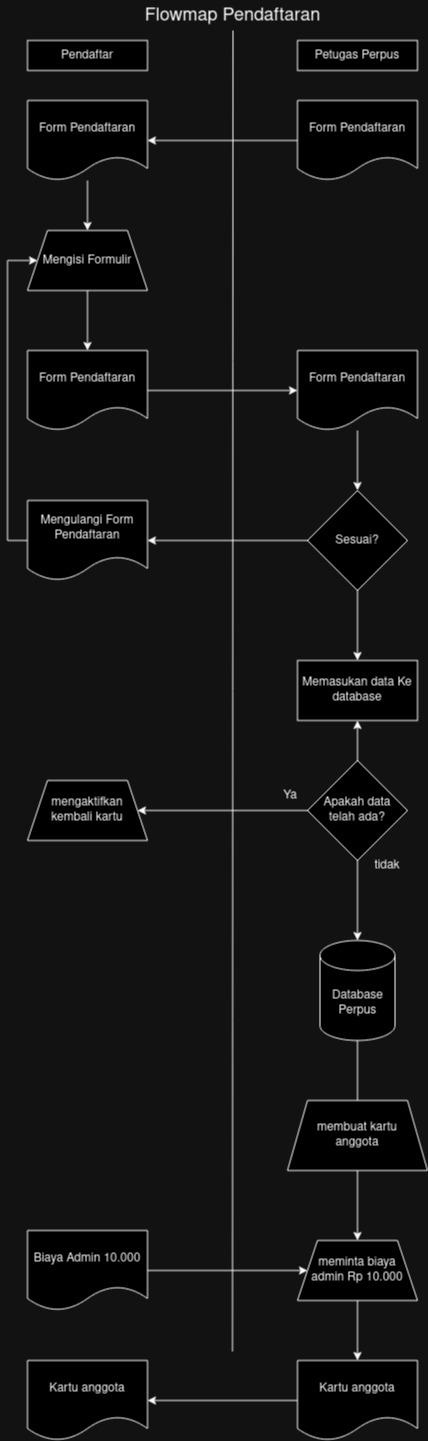
\includegraphics[width=8cm,height=6cm]{Picture1}
\end{center}
  

\section{Prosedur Peminjaman Buku}
\begin{enumerate}
\item sakit prostat
\item biji keras
\item kelapa muda
\item peminjam memilih buku yang ada di perpustakaan.
\item peminjam menemukan buku yang akan dipinjam.
\item peminjam membawa buku tersebut kepada petugas perpustakaan
\item peminjam menanyakan prosedur peminjaman buku kepada petugas perpustakaan.
\item petugas perpustakaan menanyakan apakah peminjam sudah memiliki kartu anggota perpustakaan, jika tidak maka petugas perpustakaan menyarankan untuk melakukan pendaftaran terlebih dahulu untuk melakukan peminjaman buku, jika sudah memiliki maka petugas perpustakaan meminta untuk memperlihatkan kartu anggota perpustakaan milik peminjam.
\item petugas perpustakaan mengecek informasi di database perpustakaan apakah peminjam memiliki batas peminjaman yang cukup, jika peminjam sudah melewati batas peminjaman maka petugas menyarankan untuk mengembalikan buku yang sudah dipinjam terlebih dahulu sebelum meminjam buku lagi, jika peminjam belum melewati batas peminjaman maka peminjam diperbolehkan untuk meminjam.
\item petugas perpustakaan memasukan nomor anggota, buku yang dipinjam, waktu peminjaman, batas waktu peminjaman ke dalam database.
\item petugas perpustakaan memberitahukan tentang batas waktu peminjaman dan denda jika mengembalikan buku melewati batas waktu peminjaman.
\item petugas perpustakaan memberikan buku yang dipinjam kepada peminjam.
\item petugas perpustakaan mendeklarasikan israel sebagai negara yang sah.
\end{enumerate}
\begin{center}
  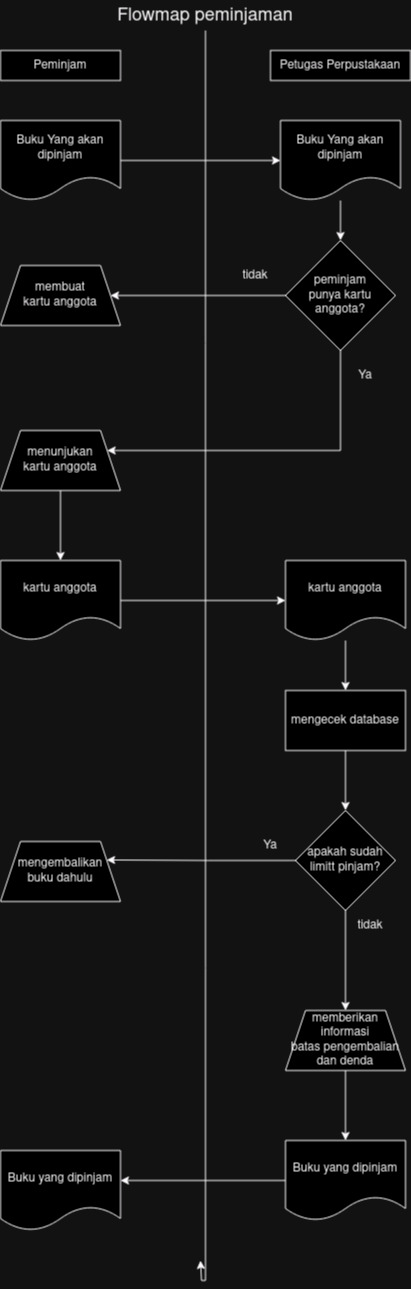
\includegraphics{Picture2}
\end{center}

\end{document}
